\section{Experimental Design}
\label{sec:experiment}

\subsection{Development/external split}

BOSSBase 1.01 (10,000 512$\times$512 grayscale images) is the development corpus used to choose the final protocol family and operating point. It is therefore not used as untouched external evidence in the headline TOMM claims. External validation uses the official Caltech-101 distribution, containing 9,144 readable source images. For each seed in $\{11,29,47,71,101\}$, a deterministic permutation assigns 1,500 images to descriptor training and the next 7,000 disjoint images to the cover index. Caltech images are converted uniformly to RGB before the 256$\times$256 channel fit.

The frozen external operating point is $K=8$, group size five, 128 parity bytes, and 30 authenticated sessions per partition. Ten deterministic plaintexts are generated at each of 8, 32, and 64 bytes; global authenticated sequences are 0--9, 10--19, and 20--29 respectively. A public deterministic benchmark root derives partition-specific keys and nonces, so the experiment is reproducible while making no production key-management claim.

\subsection{Calibration and holdout channel tests}

The twelve calibration transformations are exactly those listed in Section~\ref{sec:method}. The holdout set is never used for projection or group-bank construction and contains eight intermediate/stronger transformations: Gaussian noise 9 and 15; blur 1.2 and 1.8; central crop 8\% and 12\%; and rotations 5 and 9 degrees. Each of 30 sessions is evaluated under every transformation for each of five partitions, yielding 1,800 calibration trials and 1,200 holdout trials. Trial success requires exact authenticated plaintext recovery; a high symbol-accuracy value without successful AEAD verification is a failure.

\subsection{Selection-detectability audit}

The final detector audit reconstructs the complete 30-session selected-cover schedule for every external partition. For each partition and each of 20 repetitions, a 65/35 image-disjoint train/test split is created with split seed $10{,}000s+r$. The same split is used across all 30 session heads. We report macro-AUC across heads for three frozen detectors:

\begin{enumerate}
\item a 52-dimensional residual/SRM-lite representation with a native multi-output ExtraTrees classifier (300 trees, square-root feature sampling, balanced classes);
\item five GLCM texture features with standardized balanced logistic regression, trained independently for each session head;
\item a lightweight 30-output CNN trained for eight epochs with AdamW ($10^{-3}$, weight decay $10^{-4}$), batch size 32, and binary cross-entropy with logits.
\end{enumerate}

There are 100 repeated splits per detector. Because splits overlap within a partition, intervals over those repetitions are descriptive rather than confirmatory independent-sample confidence intervals; we do not report a naive one-sample repeated-split $t$-test.

\subsection{Frozen DiffStega reproduction}

DiffStega \cite{yang2024diffstega} is executed from official commit \texttt{73cd7cb8d102f4fc0f5bb168a71cfb948077d89a} on the official 100-case UniStega corpus (30 similar-prompt, 42 content-prompt, 28 style-prompt cases). The environment uses Python 3.11.5, PyTorch 2.1.0+cu121, CUDA 12.1, and a Tesla T4. All upstream benchmark commands and model identifiers remain frozen. The benchmark produces 700 PNG files and no evaluation error.

The upstream repository does not provide the metric-extraction scripts used for its paper tables. We therefore compute PSNR, SSIM, LPIPS, face ID similarity where applicable, CLIP score, and NIQE in an independent post-execution metric environment. Two package versions in that metric-only environment differ from the preregistered freeze (\texttt{huggingface-hub} 0.36.2 vs. 0.20.3 and \texttt{pyiqa} 0.1.15 vs. 0.1.13). Consequently, these are labeled \emph{independently reproduced metrics}; exact equality with the IJCAI table is neither expected nor claimed.

\section{Results}
\label{sec:results}

\subsection{External calibration feasibility and recovery}

All five external partitions produce feasible group banks for all 30 authenticated sessions. Across five partitions, 30 sessions, and 12 calibration attacks, all 1,800 protected messages are recovered and authenticated. Maximum Reed--Solomon corrections in any calibration trial are 37, below the 64-byte correction radius implied by 128 parity bytes. Every 7,000-cover index is exercised over the complete schedule, which avoids the trivial security failure mode of permanently restricting communication to a small fixed subset.

\begin{table}[t]
\caption{External Caltech-101 calibration results under the frozen protocol. Projection selection uses calibration evidence only.}
\label{tab:calibration}
\small
\begin{tabular}{@{}rlrrr@{}}
\toprule
Seed & Selected projection & Stable covers & Recovery & Max RS corr. \\
\midrule
11  & random\_04 & 4,184 & 360/360 & 5 \\
29  & random\_04 & 3,795 & 360/360 & 37 \\
47  & random\_15 & 4,756 & 360/360 & 0 \\
71  & random\_20 & 3,933 & 360/360 & 11 \\
101 & random\_28 & 4,167 & 360/360 & 0 \\
\midrule
All & -- & -- & 1800/1800 & 37 \\
\bottomrule
\end{tabular}
\end{table}

\subsection{Unseen holdout robustness}

The external holdout campaign recovers 1,163 of 1,200 authenticated messages (96.92\%). Failure is sharply localized: all 37 failures occur under the unseen 12\% central crop. The other seven transformations each recover 150/150 messages. This localization matters more than the aggregate alone; it identifies cropping beyond the calibration range as the dominant external-validity boundary.

\begin{table}[t]
\caption{External holdout results. Cover-label accuracy is averaged before group majority/FEC; message success requires final authenticated plaintext recovery.}
\label{tab:holdout}
\small
\begin{tabular}{@{}lrrr@{}}
\toprule
Holdout transformation & Auth. recovery & Mean label acc. & Max RS corr. \\
\midrule
Gaussian $\sigma=9$  & 150/150 & 0.964 & 0 \\
Gaussian $\sigma=15$ & 150/150 & 0.950 & 2 \\
Blur 1.2              & 150/150 & 0.958 & 0 \\
Blur 1.8              & 150/150 & 0.928 & 5 \\
Crop 8\%              & 150/150 & 0.707 & 34 \\
Crop 12\%             & 113/150 & 0.603 & 64 \\
Rotate $5^\circ$      & 150/150 & 0.923 & 0 \\
Rotate $9^\circ$      & 150/150 & 0.860 & 26 \\
\midrule
All holdouts           & 1163/1200 & -- & 64 \\
\bottomrule
\end{tabular}
\end{table}

Per-partition authenticated success is 240/240, 214/240, 240/240, 231/240, and 238/240 for seeds 11, 29, 47, 71, and 101. Thus the strongest crop exposes partition variability even though seven other holdouts are uniformly recovered.

\subsection{Selection detectability}

Table~\ref{tab:detectors} and Fig.~\ref{fig:detectors} summarize the final detector audit. SRM-lite remains essentially at chance. GLCM reveals a small, highly repeatable texture/selection shift. The trained CNN is the strongest evaluated warden, with mean macro-AUC 0.5266; every seed-level mean lies above 0.523. This is a modest but systematic signal. It falsifies any universal ``undetectable'' characterization and motivates the narrower statement that NARCIS has low detectability under the evaluated matched-index detector family.

\begin{table}[t]
\caption{Final repeated Caltech-101 selection-detector audit ($n=100$ overlapping image-disjoint splits per detector). Intervals are descriptive, not independent-sample inferential confidence intervals.}
\label{tab:detectors}
\small
\begin{tabular}{@{}lrrrr@{}}
\toprule
Detector & Mean AUC & SD & Min--Max & Descriptive 95\% interval \\
\midrule
SRM-lite + ExtraTrees & 0.5040 & 0.0023 & 0.4969--0.5088 & 0.5036--0.5045 \\
GLCM + logistic       & 0.5128 & 0.0017 & 0.5088--0.5162 & 0.5125--0.5132 \\
30-head CNN           & 0.5266 & 0.0034 & 0.5186--0.5340 & 0.5259--0.5273 \\
\bottomrule
\end{tabular}
\end{table}

\begin{figure}[t]
\centering
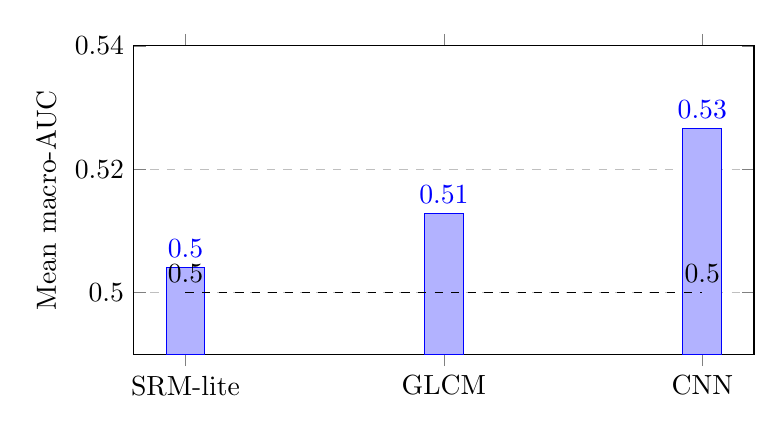
\begin{tikzpicture}
\begin{axis}[
  ybar,
  ymin=0.49,ymax=0.54,
  ylabel={Mean macro-AUC},
  symbolic x coords={SRM-lite,GLCM,CNN},
  xtick=data,
  bar width=14pt,
  width=0.78\textwidth,
  height=55mm,
  nodes near coords,
  nodes near coords align={vertical},
  ymajorgrids=true,
  grid style={dashed},
]
\addplot coordinates {(SRM-lite,0.504048) (GLCM,0.512833) (CNN,0.526603)};
\addplot[sharp plot,dashed,mark=none] coordinates {(SRM-lite,0.5) (CNN,0.5)};
\end{axis}
\end{tikzpicture}
\caption{Mean macro-AUC of the frozen detector battery. The dashed reference is chance AUC 0.5.}
\Description{Bar chart with SRM-lite at 0.504, GLCM at 0.513, and CNN at 0.527, with a dashed chance line at 0.5.}
\label{fig:detectors}
\end{figure}

\subsection{DiffStega reproduction and comparison boundary}

All 100 official UniStega cases complete under the frozen external execution. Table~\ref{tab:diffstega} compares the independently reproduced values with the published IJCAI reference. Correct-recovery PSNR is 23.274 dB, within 0.016 dB of the reported 23.290 dB. Face-ID similarity on 22 face cases is likewise close (0.888 vs. 0.893). Other metrics show larger offsets, which are retained rather than tuned away and are consistent with using an independent metric environment.

\begin{table}[t]
\caption{DiffStega external reproduction. ``Reproduced'' values are independently computed from the 100-case official execution; ``Published'' values are reported by Yang et al. \cite{yang2024diffstega}.}
\label{tab:diffstega}
\small
\begin{tabular}{@{}llrr@{}}
\toprule
Condition & Metric & Reproduced & Published \\
\midrule
Encrypted & PSNR & 18.569 & 18.611 \\
          & SSIM & 0.529 & 0.590 \\
          & LPIPS & 0.418 & 0.461 \\
          & Face ID similarity & 0.345 & 0.343 \\
          & CLIP score & 28.946 & 29.446 \\
          & NIQE & 3.901 & 3.408 \\
\midrule
Correct recovery & PSNR & 23.274 & 23.290 \\
                 & SSIM & 0.672 & 0.769 \\
                 & LPIPS & 0.183 & 0.266 \\
                 & Face ID similarity & 0.888 & 0.893 \\
\midrule
No password & PSNR & 18.495 & 18.491 \\
Wrong password & PSNR & 17.613 & 17.530 \\
\bottomrule
\end{tabular}
\end{table}

These values are not inserted into a ``NARCIS vs. DiffStega'' winner table. DiffStega's information object is a reconstructed secret image and its perceptual metrics quantify that reconstruction. NARCIS's primary outcome is exact authenticated recovery of a byte string from a finite natural-image index. Comparing PSNR with NARCIS's symbol rate or treating the two as equal-capacity systems would therefore be a category error.
